\documentclass[11pt]{jreport}
%\documentclass[11pt,twoside]{jreport} %印刷に出すときは両面見開きにするかな

\usepackage{fancyhdr}
%\usepackage{graphicx}
\usepackage[dvipdfmx]{graphicx}
%\usepackage[dvipdfm]{graphicx,color}
\usepackage{epsf}
\usepackage{url}
\usepackage{amsmath}
\usepackage{amsfonts}
\usepackage{comment}

\let\origtitle\title
\let\origauthor\author

\newcommand{\thetitle}{a}
\newcommand{\theauthor}{a}

\renewcommand{\bibname}{参考文献}

\makeatletter

\renewcommand{\chapter}{%
  \if@openright\cleardoublepage\else\clearpage\fi
  \thispagestyle{fancy}
  \global\@topnum\z@
  \@afterindenttrue
  \secdef\@chapter\@schapter
}

\makeatother

\pagestyle{fancy}

\fancyhead{}
\rhead{\footnotesize\thepage}
\lhead{\footnotesize\leftmark}
\chead{\footnotesize\rightmark}
\cfoot{}

\renewcommand{\chaptermark}[1]{\markboth{第\ \normalfont\thechapter\ 章~#1}{}}
\renewcommand{\sectionmark}[1]{\markright{\thesection #1}{}}
\renewcommand{\headrulewidth}{0.4pt}
\renewcommand{\footrulewidth}{0.4pt}
\renewcommand{\title}[1]{\lfoot{\footnotesize{#1}\origtitle{#1}}\renewcommand{\thetitle}{#1}}
\renewcommand{\author}[1]{\rfoot{\footnotesize{#1}\origauthor{#1}}\renewcommand{\theauthor}{#1}}

\begin{comment}
  \lhead[{\footnotesize\hspace{1em}\thepage\hspace{2em}\rightmark}]{}
  \rhead[]{{\footnotesize\hspace{1em}\leftmark\hspace{2em}\thepage}} %見開き用
\end{comment}

\newcommand{\athr}[1]{\author{#1}}


\renewcommand\floatpagefraction{.001}
\makeatletter
\setlength\@fpsep{\textheight}
\makeatother


%ここから
\title{複数の携帯端末による教室空間の空間音響環境構築手法の検討}
\author{14M7102\\伊納洋佑}
\date{\today}

\let\origtitle\title
\let\origauthor\author

\begin{document}

  \thispagestyle{empty}
  \begin{center}
    \vspace{1.5cm}\huge{\thetitle}\\ \vspace{3.0cm}
    \LARGE{総合情報学研究科}\\
    \LARGE{知識情報学専攻}\\
    \vspace{0.8cm}\Large{インタラクションの認知・メディア・文化}\\
    \vspace{0.8cm}\LARGE{\theauthor}\\ \vspace{1.0cm}
  \end{center}

\def\thepage{}
  %内容
  \chapter*{概要}
\addcontentsline{toc}{chapter}{概要}

%元の概要と同じ内容を貼り付けるかんじ
本論文では,納豆の糸引きを自動的に観測し,その糸の形状や太さから,繊維としての最小単位を割り出す手法を紹介し,その有効性について議論する.

  %もくじ
  \tableofcontents
  \listoftables
  \listoffigures

\pagestyle{fancy}
  \chapter{序論}


\section{緒論}

%緒論,,どのくらいかくのかな
%\clearpage
%2ページとか??4ページとか??


%\begin{figure}[tb]\centering
%\epsfxsize=10cm\epsffile{eps/nattorice.eps}
%\caption{元気の源,納豆ごはん}\label{fig:nattorice}
%\end{figure}


近年スマートデバイスの普及・通信技術の発達により,個人が各自端末を持ち歩くようになった.
このようなデバイスには,通信機能や音声入力・出力装置など様々なセンサやアクチュエータが搭載されており,デバイスを保持しているユーザに様々なサービスを提供できる.
近年はユビキタスな情報サービスとして各端末から情報を集め多数のユーザへのサービス状態を最適化するための研究もある\cite{11ubi}.
このように,多人数からのリソースと取得データを用いた多人数へのサービスが実現できるようになった.


実空間内のユーザ間でのコミュニケーション引き起こすものとして,すれ違い通信\cite{surechigai}のような個人と個人の関係性に着目したものがあるが,多くの人が存在する空間の中で多人数のコミュニケーションに着目したものは見られない.

本研究では,授業や講演,学会発表などのある程度大規模な閉鎖空間での,一人対多人数のコミュニケーションに注目した.
これまでのような話し手が一方的に聴衆に話し続けるだけのコミュニケーションではなく,疑問や未理解・不明点といった反応を,話し手および聴衆の双方に即時的にフィードバックすることで,不明点の質問に臆することが減ったり,重要個所の情報を強調的に取得出来たりするなど,よりアクティブな知的コミュニケーション空間を作ることができると考えた.

これまでにもclicker\cite{clicker}やリアルタイムアンケートシステム\cite{imakiku},twitterやchat画面への書き込みによる\cite{twitter},講義へのフィードバック手法が試みられている.
しかしこれらは視覚的情報でのフィードバックが多いため,講演や講義などの話者が中断することなくその内容を知ることはできず,結果として参加者からの意見が必須なシーンのみ活用されたり,参加者同士のコミュニケーションのみを盛り上げることになる.


\section{研究の目的}

それに対し本研究では,広い空間内にいる多人数の端末を用いた音声コミュニケーション手法として,音源定位を用いた同時多発的なやり取りを提案する.
そして,特殊な音響装置のある教室や講演スペースによらず実現するため,参加者個人の端末をスピーカアレイとして活用することを考えた.


\begin{figure}[tb]
  \centering
  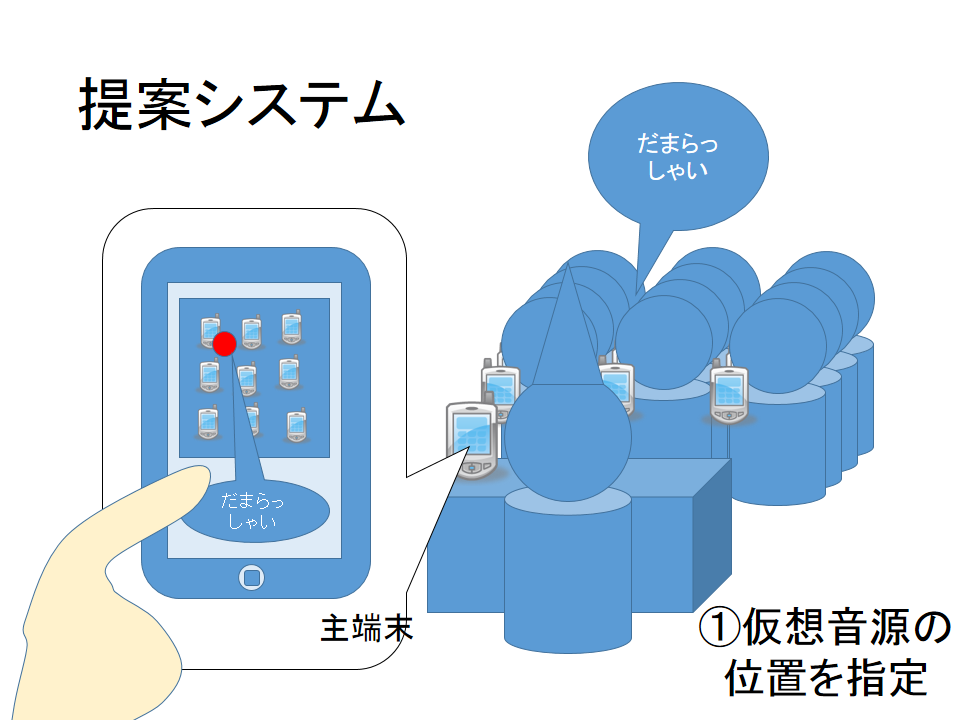
\includegraphics[clip,width=1.05\hsize]{img/shikumi1.png}
  \caption{しくみ}\label{fig:shikumi1}
\end{figure}


本稿では,これらの端末が互いの位置や時間遅れを把握し,適切な音源定位による音声情報提示を行うため,端末間の距離測および同期手法として,
直接スペクトル拡散方式による測距手法を提案する.これにより,比較的高精度な同期と端末間の距離計測が行われる.音源定位を指定した音声情報提示の際には,端末間距離情報が,
どの端末を用いるか,
また,どの程度の振幅パニングにより音源位置を設定するか
に用いられる.

これにより,特定多数のユーザによるパラレルコミュニケーションの実現だけでなく,駅構内や避難所などの不特定多数のユーザがいる空間においても,適切に音源定位した音声情報提示を行うことができるようになると期待される.



%ここはかなり大事
\clearpage
%わかりやすく,段落を丁寧に区切りましょう

%\section{本論文の構成}

  \chapter{関連研究}
%または
%\chapter{菌類}

\section{位置情報に基づく情報提供}

複数のスマートデバイスで複数のユーザにサービスを提供するシステムとして,
位置情報を利用した携帯端末への音声情報配信\cite{kawagoe14}がある.
このようなサービスは,
ユーザ情報を取得し共有するための
個人を対象としたサービスであり,集団を対象とはせず,
端末間の通信で実空間に刺激を形成するものでもない.


\section{マルチチャンネルスピーカ}

これまでの多チャンネルスピーカによる音場再現手法としては,
波面合成法(WFS: wave field synthesis)\cite{wfs, 木村敏幸},
高次アンビソニックス法(HOA: higher order Ambisonics)\cite{hoa, 小山翔一},
境界音場制御法\cite{sfc, 伊勢史郎, 岡田耕介},
などが知られている\cite{鈴木陽一, 濱崎公男, 尾本章}.
また,パラメトリックスピーカを用いて特定の場所に音像を定位する手法\cite{paramsp}がある.
他にも,複数のスピーカを用いて振幅パンニングをするVector-base Amplitude Panning(VBAP)法\cite{PULKKI}や
Distance-based Amplitude Panning(DBAP)\cite{dbap}がある.
さらに,ユーザが移動しても音像を提供することができる手法\cite{湯山雄太}なども開発されている.
しかし,これらの手法はどれも特殊な機器と特別な設定が必要であり,
公共空間への導入が困難である.



\section{アドホックマイクロホンアレイ}

端末間同期手法に関して,
音の発信を利用したスマートフォンアレイの機器位置推定\cite{shibata13}や
音の発信を利用したキャリブレーションに基づくアドホックマイクロホンアレイによる音源位置推定\cite{shibata14}がある.
マイクロホンアレイは複数スマートデバイスのマイクロホンで取得した多チャネル信号を処理し,音源位置推定,音源分離などを行う\cite{小野順貴14-1, 小野順貴14-2}.
これはスマートデバイスでアレイ処理をする点においては似ているが,
本研究ではスピーカアレイを構築するために相対位置推定や同期を行うためのマイクロフォンの利用という点で異なる.

また,端末間での音声による同期手法としては センサネットワークによる音声同期手法 \cite{SYED, XU} や,
水中センサネットワークでの音響通信 \cite{LU, AKYILDIZ, 浜田龍平},
それを応用したスマートフォン間での同期手法 \cite{PENG, LAZIK, ENS, JANSON} が提案されている.



\section{信号検出}

本論文で利用する信号処理用語についても触れておく.

\subsection{フーリエ変換}
受信信号には目標信号と雑音成分が含まれている.
その波形は様々な周波数と振幅と位相の異なる正弦波の和として表現することができる.
正弦波の和として表した波形を解析するためにフーリエ変換という手法が使われている.
波形を周波数.振幅.位相で表現する方法を,時間領域波形 $x(t)$ の周波数領域表現 $X(\omega)$ という.
$X(\omega)$ は波形 $x(t)$ のスペクトルと呼ばれる.
時間領域から周波数領域への変換をフーリエ変換と呼び,周波数領域から時間領域への変換は逆フーリエ変換と呼ばれる.
フーリエ変換とフーリエ逆変換を次のように定義される.
$$\begin{aligned}
\mathcal{F}[x(t)] & = X(\omega) = \int^{\infty}_{-\infty} x(t) e^{-j\omega t}dt \\
\mathcal{F}^{-1}[X(\omega)] & = x(t) = \frac{1}{2\pi} \int^{\infty}_{-\infty} X(\omega) e^{j\omega t}d\omega
\end{aligned}$$
互いにフーリエ変換と逆変換の関係になっているものをフーリエ変換対という.

\subsection{相関関数}
受信信号は目標信号と雑音が混在する不規則信号である.
時刻 $t$ における不規則信号 $x(t)$ とさらに時間 $\tau$ だけ経過した不規則信号 $x(t+\tau)$ との相関は
$$\begin{aligned}
\phi(\tau)
&= \lim_{T\to \infty} \frac{1}{2T} \int^{T}_{-T} x(t) x(t+\tau)dt \\
\end{aligned}$$
と定義される.
$\phi(\tau)$ を自己相関関数という.
自己相関関数は $\tau=0$ のとき,つまり自分自身の波形の積をとったときに最大値を取る偶関数である.
自己相関関数は波形の周期を調べるのに使われ,波形が周期的ならば,その自己相関関数も同じ周期でピークを示す.

2つの不規則信号波形の一方を $\tau$ だけ遅延させたときの相関関数を相互相関関数と呼び,
$$\begin{aligned}
\phi_{xy}(\tau)
&= \lim_{T\to\infty} \frac{1}{2T} \int^{T}_{-T} x(t) y(t+\tau)dt
\end{aligned}$$
で定義される.
相互相関関数は2つの信号間の類似度や時間遅れの測定に利用される.
もし,完全に異なった信号ならば $\tau$ の位置に関わらず相互相関関数は $\phi_{xy}(\tau)=0$ である.

元信号をフーリエ変換したものの絶対値の二乗 $X(\omega) \overline{X(\omega)}$ と相関関数はフーリエ変換対である.
つまり,元信号 $x(t)$ をフーリエ変換して得られた $X(\omega) \overline{X(\omega)}$ を逆フーリエ変換すると相関関数となる.
\[\xymatrix{
    x(t) \ar[r]^{相関関数} \ar[d]_{\mathcal F}
  &
    \phi(\tau)
\\
    X(\omega) \ar[r]_{\left|\cdot\right|^2}
  &
    \Phi(\omega)=X(\omega) \overline{X(\omega)} \ar[u]_{{\mathcal F}^{-1}}
}\]
これを Wiener-Khintchine の定理という.
この定理を利用すると,自己相関関数および相互相関関数の計算に高速フーリエ変換(FFT:Fast Fourier transform)を利用することができるので,
直接相関関数を計算するよりも計算量を削減することができる.


\subsection{整合フィルタと相関処理器}
雑音を含む入力信号に対してピーク値のSN比(signal to noise ratio)を最大にするフィルタを
整合フィルタ(matched filter)という.
整合フィルタを作成するには送信信号の波形がわかっている必要があり,
実用上は整合フィルタと相関処理器は等しい.
つまり雑音成分 $n(t)$ を含む信号 $y(t)=x(t)+n(t)$ に対して,
元の信号 $x(t)$ との相互相関 $\phi_{xy}(t)$ を求める処理は整合フィルタになる.

\subsection{曖昧度関数}
レーダーやソーナー信号処理において,
使用目的や環境にあわせて,どのような信号を使用すれば,
雑音や残響と分離しやすく,
周波数分解能や時間分解能を向上させることができるか,の指標として,
曖昧度関数がある.
曖昧度関数 $Q(\tau, f_d)$ は不確定性関数 $|\chi(\tau, f_d)|$ を二乗したものである.
不確定性関数は時間遅延 $\tau$ と 周波数シフト $f_d$ 変化した信号と元信号の相関関数である.
$$\begin{aligned}
Q(\tau, f_d)
&= |\chi(\tau, f_d)|^2 \\
&= \left|\int_{-infty}^{\infty}x(t)\overline{x(t+\tau)} e^{j2\pi f_d t}dt\right|^2
\end{aligned}$$
曖昧度関数および不確定関数は送信信号と受信信号の間のミスマッチに対する敏感さを表している.


\subsection{パルス圧縮手法}

信号検出においてSN比を最大化するフィルタを整合フィルタと呼び(図\ref{fig:matched_filter}),
それは元信号との自己相関に等しい\cite{seigoufilter}.
理想的には整合フィルタを通した結果がDiracのデルタ関数に近いことが望ましい.
しかし,そのような信号は短時間に大電力のパルスとなるため,送信機器の送信電力や回路の容量に物理的な制約があるため,
そのような信号の送信は不可能である.
そこで,パルス圧縮と呼ばれる手法が使われている\cite{pulsecompress}.
パルス圧縮は,送信パルスを時間方向や周波数方向へエネルギーを拡散させ,
受信時にフィルタと高SN比で鋭いピークを持つようにする手法である.
特に,周波数方向へ拡散させる変調方式をスペクトル拡散変調と呼ぶ(図\ref{fig:DS}).
レーダー\cite{レーダ技術, レーダ信号処理技術, 稲葉敬之11}およびソーナー\cite{山口功, acoima, 海洋音響の基礎と応用, 水中音響学},
そして通信\cite{高野忠00, 高野忠01}の分野において,信号パルスの信号対雑音比を向上させるために,パルス圧縮は使われている\cite{電子戦の技術基礎編, 電子戦の技術拡充編, 電子戦の技術通信電子戦編}.
パルス圧縮手法には,チャープ信号と呼ばれる時間に対して周波数が線形に変化する信号や,Barker符号.M系列符号などの拡散符号が用いられる\cite{谷本正幸, specto, yamauchi, Dixon}.
これらの技術は音響におけるインパルス応答測定にも利用されている\cite{渋澤功, 金田豊, 守谷直也, nonlinear}.

\begin{figure}[p]\centering
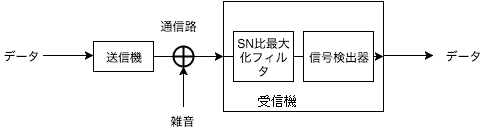
\includegraphics[clip,width=1.05\hsize]{img/matched_filter.png}
\caption{送受信モデルと整合フィルタ}\label{fig:matched_filter}
\end{figure}


\begin{figure}[p]\centering
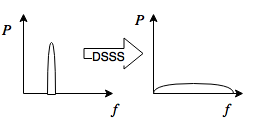
\includegraphics[clip,width=1.05\hsize]{img/DS.png}
\caption{スペクトル拡散によるパルス圧縮}\label{fig:DS}
\end{figure}


\subsection{チャープ信号}

周波数を時間に比例して変化させた波をチャープ信号(Chirp Signal)という.
波形を図\ref{fig:chirpsig}に示し,スぺクトログラムを図\ref{fig:chirpsig2}に示す.
チャープ信号は線形周波数変調(LFM: Linear Frequency Modulated)信号とも呼ばれる.
また,インパルス応答測定の分野においては時間引き伸ばしパルス(TSP: Time Stretched Pulse)とも呼ばれる\cite{Aoshima},.
チャープ信号は,方形パルスを周波数方向へ掃引することで,図\ref{fig:chirppulse_amb}に示すように,
通常パルスと同じ電力で時間方向の精度を向上させることができる(図\ref{fig:chirppulse_amb}).
チャープ信号は受信波形と送信波形との相互相関を求めることにより,
通常の反射波形に変換された信号が得られる.
チャープ信号によるパルス圧縮は,
相関処理により信号を検出するので,
通常のパルス型の音源に比べて
雑音の影響を受けにくいという利点がある.
また,パルス型の音源に比べ瞬間のエネルギーは小さいが,
送波時間を長くすることにより,
相関後のエネルギーを通常パルスよりも大きくすることができるというパルス圧縮の効果が得られる.
チャープ信号はレーダーやソーナー,インパルス応答の測定に利用されている.


\begin{figure}[p]\centering
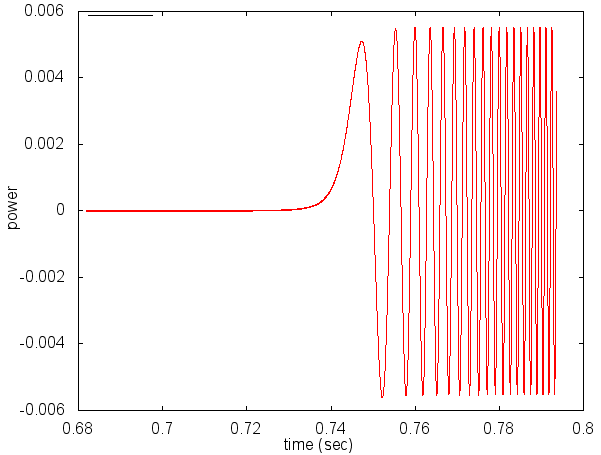
\includegraphics[clip,width=1.0\hsize]{img/chirp.png}
\caption{チャープ信号波形}\label{fig:chirpsig}
\end{figure}

\begin{figure}[p]\centering
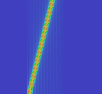
\includegraphics[clip,width=0.7\hsize]{img/chirp_spectogram.png}\\
\caption{チャープ信号スぺクトログラム}\label{fig:chirpsig2}
\end{figure}


\begin{figure}[p]\centering
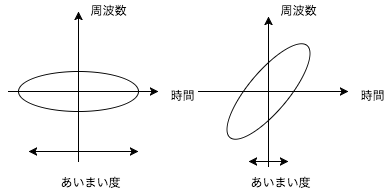
\includegraphics[clip,width=0.9\hsize]{img/aimai.png}\\
通常パルス~ ~ ~ ~ ~ ~ ~ ~ ~ ~ ~ Chirpパルス
\caption{通常パルスとチャープパルスによる曖昧度の比較}\label{fig:chirppulse_amb}
\end{figure}



\subsection{PSK信号}
チャープ信号はドップラー効果の周波数ずれに対してパルス位置が変わるだけで,サイドローブは劣化しにくい.
しかし,継続時間の長いチャープ信号は曖昧度関数のピーク周辺のサイドローブが大きくなるため,
非常に遠距離間での信号検出や,雑音が大きな環境間での微弱な信号検出には,
継続時間を伸ばしても性能が劣化しにくいM系列符号やそれを応用した符号系列を用いた
直接スペクトル拡散(DSSS: direct sequence spread spectrum)が用いられる.
直接スペクトル拡散変調は,位相偏移変調方式(PSK:Phase-shift keying)により,ビット系列で正弦波を変調する.
特に,正弦波の位相を0と $\pi$ に変化させ,それぞれ1と-1を割り当てる場合,
2値符号変調方式(BPSK:Binary Phase-shift keying)という.
PSC信号では,チャープ信号と同じく通常パルスと比べ.
パルス幅を長く保ったまま時間分解能を上げることができる.
また,ビット系列の選び方によって相関処理後のサイドローブが変化する.
サイドローブを抑える系列として,バーカー符号とM系列符号がある.
PSK信号とチャープ信号とを比較すると,
PSK信号は対象物が移動してドップラー効果が生じるような場合には,サイドローブが劣化しやすく,
また,非線形な歪みを生じることがある.

\begin{figure}[p]\centering
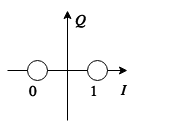
\includegraphics[clip,width=0.27\hsize]{img/chirp_qi.png}
\caption{BPSK信号空間ダイヤグラム}\label{fig:chirpqi}
\end{figure}

\subsection{バーカー符号}
バーカー符号(Barker code)(図\ref{fig:barkercode})は直接スペクトル拡散変調によるパルス圧縮に用いられる符号系列の一種である.
同期点以外での自己相関関数の絶対値の最大が$1/N$となる長さ$N$の有限長系列で,長さ13まで存在し,
相関特性が長さ13の場合,ピークが13倍,サイドローブが1/13倍となるような,
ディラックの$\delta$関数に近い理想的な相関特性を持つ.

バーカー符号はサイドローブをできるだけ小さくするような符号列であり,
サイドローブがすべて $1/N^2$ になる系列である.
バーカー符号は $N=13$ までしか知られていないが,
さらにパルス圧縮して時間分解能を上げたい時は,M系列符号を使う.
バーカー符号はレーダーやソナー,ロケットのトランスポンダ\cite{高野忠00}など利用されている.

\begin{figure}[p]\centering
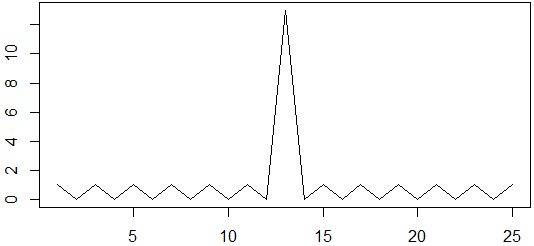
\includegraphics[clip,width=0.9\hsize]{img/barkercode.png}
\caption{Barker符号(13列)の自己相関}\label{fig:barkercode}
\end{figure}

\begin{table}[p]\centering
  \caption{バーカー符号の種類とサイドローブレベル}
  \label{tab:barker}
  \begin{tabular}{l|ccc}
    \hline
    長さ N & 系列 $\{q_n\}$ & サイドローブ[dB] \\
    \hline
    2  & 1,-1 | 1,1                   & -6.0 \\
    3  & 1,1,-1 | 1,1                 & -9.5 \\
    4  & 1,1,-1,1 | 1,1,1,-1          & -12.0 \\
    5  & 1,1,1,-1,1                    & -14.0 \\
    7  & 1,1,1,-1,-1,1,-1              & -16.9 \\
    11 & 1,1,1,-1,-1,-1,1,-1,-1,1,-1   & -20.8 \\
    13 & 1,1,1,1,1,-1,-1,1,1,-1,1,-1,1 & -22.3 \\
    \hline
  \end{tabular}
\end{table}



\subsection{M系列符号}
最大周期シフトレジスタ(Maximum length shift register)系列は,M系列とも呼ばれ,
線形帰還シフトレジスタ(LFSR: Linear feedback shift register)を使って生成される擬似雑音(PN)系列の一種である.
LFSRとは,図\ref{fig:LFSR}のような排他的論理和による帰還タップを持つシフトレジスタである.
バーカー符号が有限の符号系列であるのに対して,M系列符号は有限の符号系列が周期的に繰り返される.
M系列は.LFSRに全てゼロ以外の初期値を与えることにより生成される周期系列のうち,
周期 N が最大となるものである.
1周期中に全ゼロ以外の全ての k ビットパターンが必ず1回出て来くるので,$N=2^k-1$ となる.
このような系列はLFSRの帰還結線の位置がある限られた組み合わせを満たすときのみ生成され,
それ以外の場合は周期のより短い系列となる.
M系列の系列の長さNが十分に長いとき,
曖昧度関数のサイドローブの最大値は $1/N$ となる\ref{fig:mseqautocorrel}.
M系列符号は系列を長くしてもサイドローブを抑えることができるという特徴から,
微弱信号の検出が必要とされる深宇宙探査機との通信\cite{dsn}や海洋音響トモグラフィ\cite{tomography}などに使われている.
また,初期値が異なるM系列どうしの相互相関は直交しピークを持たないという性質から,
通信分野において符号分割多元接続(CDMA:Code Division Multiple Access)に利用される.

\begin{figure}[p]\centering
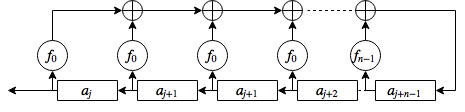
\includegraphics[clip,width=0.9\hsize]{img/M-sequence.png}
\caption{LFSRのブロック線図}\label{fig:LFSR}
\end{figure}


\begin{figure}[p]\centering
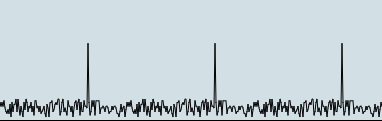
\includegraphics[clip,width=0.9\hsize]{img/mseq_autocorrel.png}
\caption{M系列をBPSK変調した波形の自己相関}\label{fig:mseqautocorrel}
\end{figure}


\section{本研究のスタンス}

以上をまとめると,
スマートデバイスを用いた情報提供システムには,個人向けの研究が目立つ.
また,複数端末を用いてマイクロホンアレイを構築する研究は存在するが,複数端末を用いてのスピーカアレイを構築する手法は比較的未開拓分野と言える.
そして,複数のスマートデバイスを用いて実空間内の複数の人間に働きかける,という本研究のシステムは,
今後さらに生活空間にスマートデバイスが普及することを考えると,
パラコミュニケーションを実現する手段としても重要であると言える.


%\section{菌類とは}
%\section{細菌類とは}
%\section{納豆菌とは}
%\section{納豆菌の既知の効能}
%\section{本研究のスタンス}

  %\chapter{納豆菌の菌糸直径計測および菌糸本数推定手法}
%\section{納豆菌の直径計測手法}
%\section{納豆菌の菌糸本数推定手法}

\chapter{提案システム}

提案システムでは,教室などの閉鎖空間において,
個人が所有する複数のスマートデバイスの音声出力をネットワークを介し同期させ制御することで,スピーカアレイを構築する.
空間内に配置した仮想音源の位置に基づき,その音源位置を囲む最寄りの3つのスマートデバイス(ノード)を設定し振幅パニングすることで,現実世界における想定位置で音源を鳴らして定位する.
このようなスピーカアレイを構築するにあたり,実空間に分布する複数のスマートデバイスの相対位置を推定するとともに,端末間での時刻同期が必要不可欠である.

%![](img/shikumi3.png)

この章では,まず,提案システムで用いた
相対位置に基づく音像定位手法について触れる.
次に,その手法を実現するための
端末間の音声パルスの到達時間差による
時刻同期手法および相対距離計測手法,
そして相対位置推定手法を述べる.
さらに,パルス圧縮を用いた信号検出手法を示し,
最後に,スピーカアレイ全体の制御手法について解説する.

\section{DBAP法を用いた音像定位}

はじめに,複数のスマートデバイスを使ってどのように音像定位するのかについて述べる.
今回のような平面配置のスピーカアレイを用いて音像定位をする手法として,
Distance-based amplitude panning (DBAP) 法がある.

- Lossius, Trond, Pascal Baltazar, and Théo de la Hogue. DBAP–distance-based amplitude panning. Ann Arbor, MI: MPublishing, University of Michigan Library, 2009.

DBAP法は,
任意の数のスピーカの位置が既知であり,
端末間のスピーカの出力特性が等しいとしたときに,
仮想音源と各スピーカとの距離から距離減衰を計算することで,
各スピーカの振幅を制御して音像を合成する手法である.

位置 $(x_s,y_s)$ にある仮想音源 $VS$ から,
位置 $(x_i,y_i)$ にある端末 $i$ への距離 $d_i$ を次のように定義する.

%![](img/DBAP.png)

$$
d_i = \sqrt{(x_i - x_s)^2 + (y_i - y_s)^2} \qquad (\mathrm{for}\ 1 \leq i \leq N)
$$

DBAP法では,仮想想源の位置に関係なく,各スピーカからの音の強さの合計は

$$
I = \sum_{i=1}^N v_i^2 = 1
$$

として正規化している.
$i$ 番目のスピーカの相対的な振幅は距離に反比例するので

$$
v_i = \frac{k}{d_i^a}
$$

と定義できる.
$k$ はすべてのスピーカと仮想音源の位置に依存した係数で,

$$
k = \frac{1}{\sqrt{\sum_{i=1}^N \frac{1}{d_i^{2a}}}}
$$

である.
係数 $a$ は距離減衰係数で

$$
a = \frac{R}{20 \log_{10}2} \\
$$

と定義する.
$R$ はロールオフ係数で,受聴者と音源の距離に基づく減衰の量である.
$R=6\ [\mathrm{dB}]$ の場合は,
自由空間における距離減衰の逆二乗則に基づき,音の強さのレベルが音源からの距離が2倍になるごとに6dBずつ減少することを意味する.
また,半自由空間では $R=3\sim5\ [\mathrm{dB}]$ 程度となる.

以上のとおり,
複数のスマートデバイスが
同期的に制御でき,
端末の位置が判明しており,
端末間のスピーカの出力特性が均一であれば,
この手法を用いて音像定位ができることが分かった.

\section{時刻同期と測距}

基準となる時刻が違う二つの時間軸を持つ端末間において同期するには,
互いに音声パルスを出せばよい.

%![](img/beeptobeep.png)

この手法はTPSN(time-sync Protocol for sensor network)

- Ganeriwal, Saurabh, Ram Kumar, and Mani B. Srivastava. "Timing-sync protocol for sensor networks." Proceedings of the 1st international conference on Embedded networked sensor systems. ACM, 2003.

などで提案されている.
原理を説明する.

端末 $A$ が自身の時刻 $t_0$ に音声パルスを発生すると,
そのパルスは音速で空間に広がり,
端末 $B$ 内の時刻 $t_1$ に受信される.
さらに,端末 $B$ からも端末 $B$ 内の時刻 $t_2$ に音声パルスを発すると,
このパルスも音速で空間に広がり,
端末 $A$ 内の時刻 $t_3$ に受信される.
ここで,図の通り,
端末 $A$ 内のパルス時間間隔 $t_3-t_0$ と
端末 $B$ 内のパルス時間間隔 $t_2-t_1$ には差が生じる.

%![](img/clock_synchronization.png)

パルスの往復で伝播にかかった時間は共に等しいと仮定すると,

$$
t_0' = t_1 - \frac{(t_3 - t_0) - (t_2 - t_1)}{2} \\
$$

となり,端末 $B$ 内時刻で端末 $A$ のパルスが発せられた時刻を推定することができる.
以上が時刻同期の原理である.

音速を $c$ とすれば,副次的に端末間の距離も求まる.

$$
d_{AB} = \frac{(t_3 - t_0) - (t_2 - t_1)}{2c}
$$

端末AB間で何らかの処理を同期的に実行したい場合は
図のようにして実行すべき時間を求められる.

%![同期実行](img/flowchart3.png)

基準となる端末Aのパルスの受信時間およびその信号の伝達時間と,
それを受信してからの経過時間 $S$ をもとに,同期的に処理を実行できる.

こうして,端末間の時刻同期と距離測定ができた.

\section{相対位置推定}


次に,複数のスマートデバイスの空間分布をどう推定するかについて述べる.
先述のとおり,端末間の相対距離は判明している.
次の非線形最小二乗法で定式化し誤差関数を最小化する最適化問題を考える.

$$
\varepsilon(\hat{x_1}, \dots, \hat{x_N}) = \sum_{i=1}^N \sum_{j\in M(i)} \left( \| \hat{ x_i } - \hat{ x_j } \| - d_{ij} \right)^2 \\
%\DeclareMathOperator*{\argmin}{arg\,min}
(\hat{x_1} \dots \hat{x_N}) = \mathrm{argmin} \varepsilon(\hat{x_1} \dots \hat{x_N})
$$

ここで,
$N \in \mathbb{N}$ は端末の数,
$M(i) \subset \{1,\dots,N\}$ は端末 $i$ と相対距離が計測できた端末の集合,
$d_{ij} \in \mathbb{R}$ は実際に計測された端末の距離とし,
$\hat{ x_i } \in \mathbb{R}^2$ n番目の端末の位置推定値で,初期値は乱数を置く.

この問題は非線形最小二乗法と言え,
最急降下法を使って反復的に解く.更新式は次のようになる.

$$\begin{aligned}
\hat{x_i} (n + 1) & = \left. \hat{x_i} (n) - a \frac{\partial \varepsilon}{\partial \hat{x_i}} \right|_{\hat{x} = \hat{x}(n)} \\
\frac{\partial \varepsilon}{\partial \hat{x_i}}
&= \sum_{j\in M(i)} \frac{\partial \left( \|\hat{ x_i } - \hat{ x_j }\| - d_{ij} \right)^2}{\partial \hat{x_i}} \notag\\
&= 2 \sum_{j\in M(i)} \left( \| \hat{x_i} - \hat{x_j} \| - d_{ij} \right) \frac{\partial \| \hat{x_i} - \hat{x_j} \|}{\partial \hat{x_i}} \notag\\
&= 2 \sum_{j\in M(i)} \left( 1 - \frac{d_{ij}}{\| \hat{x_i} - \hat{x_j} \|} \right) \left( \hat{x_i} - \hat{x_j} \right).
\end{aligned}$$

$n$ は反復回数, $a$ は更新式のステップ幅である.

端末 $i$ が測距できた他の端末の集合 $M(i)$ は後述する信号検出により決まる.

\section{信号検出}

精密な測距・時刻同期のためには精密な信号検出が必要である.
信号検出の誤差は
スマートデバイスのサンプリング周波数は44100Hz
として
1サンプルあたりの時間解像度は約 1/44100 = 22.6μs
であるので,
1サンプルあたりの距離解像度は 22.6μs*340m/s=7.7mm(音速340m/sと仮定)
である.

人間の聴覚特性として,第一波面の法則という現象が知られている.
これは二つの音源からの音声が互いに50ms以上ずれると別の音源として知覚されるというものである.

- (After Helmut Haas's doctorate dissertation presented to the University of Gottingen, Gottingen, Germany as "Über den Einfluss eines Einfachechos auf die Hörsamkeit von Sprache;" translated into English by Dr. Ing. K.P.R. Ehrenberg, Building Research Station, Watford, Herts., England Library Communication no. 363, December, 1949; reproduced in the United States as "The Influence of a Single Echo on the Audibility of Speech," J. Audio Eng. Soc., Vol. 20 (Mar. 1972), pp. 145-159.)

この場合許容される誤差は
$\pm$ 50msの誤差におよそ $\pm$ 2205サンプル以内とかなり緩いものになる.
しかしながらこれでは距離誤差が $\pm$ 3.4m ととても大きなものになってしまう.
というわけで許容される誤差は音像定位よりもむしろ距離測定の手法によって定められる.
今回のような室内空間であれば,
$\pm$ 50cmの誤差つまり $\pm$ 64サンプル以内でパルスを同定できればよいとする.

そこで,そのような高精度のパルス検出をするため,
直接スペクトル拡散方式によるパルス圧縮で高いSN比を向上させ,
信号検出には通常の整合フィルタではなくピークを尖らせることができる,
フェイズオンリー整合フィルタを利用した.

%![](img/POF.png)

$$
\begin{aligned}
\mathrm{POF}[x_a, x_b]
&= \mathcal{F}^{-1}\left[\frac{\mathcal{F}\left[x_a(t)\right]^*}{|\mathcal{F}\left[x_a(t)\right]|}\mathcal{F}\left[x_b(t)\right]\right] \\
&= \mathcal{F}^{-1}\left[\frac{X_a^*(\omega)}{|X_a(\omega)|}X_b(\omega)\right]
\end{aligned}
$$

- Horner, Joseph L., and Peter D. Gianino. "Phase-only matched filtering." Applied optics 23.6 (1984): 812-816.

直接スペクトル拡散方式による測距システムの変復調方式を図に示す.

%![](img/DS.png)

%![ブロック線図](img/DME2.png)

%![](img/DSSS.png)

搬送波には1000Hzサイン波を,拡散符号にはM系列を用い,変調にはバイナリ位相シフトキーイング(BPSK)を使った.

復調した受信信号が雑音か有効な信号かを決定する処理を信号同定という.
伝送路における伝達関数 $H(\omega)$ において室内残響の影響
としてマルチパスによるを受けてしまう.

%![](img/multipath.png)

そこで,同期パルスを測距用信号と,伝搬路を測定する参照波としてのサウンダ(sounder)信号の二つに分離した.
同期パルスから $n$ 秒後にサウンダ信号を送り,
その二つの信号の相関を取ることで,
背景雑音とは別にパルス位置を特定することが可能になる.

%![](img/sounder.png)

さらにサウンダ信号と測距信号は互いに異なる同周期のM系列を用いた.
サウンダ信号と測距信号を判別しやすくするためである.

この時刻が $n$ 秒ずれた二つの信号に対して時間窓で区切って相互相関をとることで,
信号が最も相関している区間,つまり信号の位置を特定することができる.
最後に,その区間相関値を閾値処理することで信号の到来を決定する.
今回は最大相関値前方での40%の相関値を超えたピークを到来時刻としている.

相関関数の計算にはウィーナー=ヒンチンの定理を使い周波数領域での複素乗算としてFFTを使って計算することで計算量を減らすことができる.
長さの異なる信号の高速フーリエ変換には重畳加算法を使った.

- Rabiner, Lawrence R., and Bernard Gold. "Theory and application of digital signal processing." Englewood Cliffs, NJ, Prentice-Hall, Inc., 1975. 777 p. 1 (1975).


\section{システムクロック校正}

端末のシステムクロックの進みかたはハードウェアごとに微妙に異なる.
そのため,同期してから長時間経つと,次第に端末間で遅延が生じる.
このことは,同一音源を同期的に再生し続けると,次第にずれが聞き取れるようになってくることを意味する.
この遅延を検出する手法について述べる.

端末 A のクロックを $S_A$,
端末 B のクロックを $S_B$ して,
時刻 $t$ 後に
A のサンプル数が $i$ ,
B のサンプル数が $i+d$ だけ異なっているとする.
このとき,Aを基準とした遅延比率 $S_B/S_A$ を求めたい.

%![](img/phase_shift2.png)

図より

$$\begin{aligned}
\frac{i}{S_A} &= \frac{i+d}{S_B} = t \\
\frac{S_B}{S_A} &= \frac{i+d}{i}
\end{aligned}$$

である.
遅延の検出においては,端末間の相対距離に変化がない限り,
端末Aが端末Bへとパルスを発生するだけで良く,
端末BはAへと返答パルスを返す必要はない.
既に同期済みでありAからBへの伝搬時間は算出済みだからである.

\section{音圧校正}
スマートデバイス毎にマイクロホンやスピーカのアンプ出力は異なるため,そのままではDBAP法は使えない.
ここでは,機器ごとの音圧を校正する手法を示す.

LTI(線形時不変)システムを仮定する.
$N$ 台の端末の番号を $i,j \in \{1\dots N\}$ とする.
端末 $i$ から端末 $j$ への信号伝達を考える.
$e$ を端末 $i$ で生成した単位振幅,
$v_i$ を端末 $i$ のスピーカアンプの増幅係数,
$m_j$ を端末 $j$ のマイクロホンアンプの増幅係数,
$d_{ij}=d_{ij}$ を $ij$ 間の測定距離,
$x_{ij}$ を $j$ が観測した $i$ からの信号の振幅とする.
音波の振幅は距離に反比例して減衰することが知られているので,
音声信号の伝達は

%![](img/sound_pressure_calibration.png)

$$
e v_i \frac{1}{d_{ij}} m_j = x_{ij}
$$

とモデル化できる.
このとき,ある端末 $k$ の出力係数 $v_k$ と他の端末 $i$ の出力係数 $v_i$ との比 $v_i/v_k$ を求めたい.

$$
e v_i m_j = x_{ij}d_{ij}
$$

なので

$$\begin{aligned}
\frac{e v_j m_j}{e v_k m_j} &= \frac{x_{ij} d_{ij}}{x_{kj} d_{kj}} \\
\frac{v_j}{v_k} &= \frac{x_{ij} d_{ij}}{x_{kj}d_{kj}} \\
\end{aligned}$$

である.
観測した振幅 $x_{ij}$ および測定距離 $d_{ij}$ は誤差を含むので,
それらを平均した $\hat{v_i}$ は

$$
\frac{\hat{v_i}}{v_k} = \frac{1}{N} \sum_{i\neq j \neq k} \frac{x_{ij} d_{kj}}{x_{kj}d_{ij}} \\
$$

と定義できる.$d_{ii}$ のときは距離が0となりゼロ除算が発生するので,
$i\neq j \neq k$ としている.

一番出力の低い端末 $k$ の出力係数 $v_k$ を基準とすることで,
すべての端末において定格出力を守ることができる.

\section{隣接ノードでない端末間の同期,音圧校正,クロック校正}


互いに互いの信号を検出できなかったノード間での校正を考える.
図に隣接ノードではない端末を含むネットワークを示す.

%![](img/network_topology.png)

このとき端末 A と端末 C 間では同期・測距ができていないが,
互いに端末 B とは同期・測距できているという状況である.

\subsection{同期}

時刻の基準となる
端末 $A$ がパルスを発した時間を $t_{AA}$ として
そのパルスが端末 $B$ に届いた時間は $t_{AB}$ とする.
また,
端末 $B$ がパルスを発した時間を $t_{AB}$ として
そのパルスが端末 $C$ に届いた時間は $t_{BC}$ とする.
そしてそれぞれの伝達時間を $d$ とすると図のようになる.

%![](img/rel_delay.png)

このとき,まず端末 $C$ は端末 $B$ と同期して,
その後端末 $B$ と端末 $A$ の時刻ずれ情報をもとにさらに端末 $A$ との同期ができる.


\subsection{音圧校正}

端末 $A$ を基準に音圧校正を考えると

$$
\frac{v_B}{v_A} = \frac{x_{iB} d_{iB}}{x_{AB}d_{AB}} \\
\frac{v_C}{v_B} = \frac{x_{iC} d_{iC}}{x_{BC}d_{BC}} \\
$$

であるので

$$
\frac{v_C}{v_A} =
\frac{v_B v_C}{v_A v_B} =
\frac{x_{iB} x_{iC} d_{iB} d_{iC}}{x_{AB} x_{BC} d_{AB} d_{BC}}
$$

とすれば端末 A と端末 C の出力比率を求められる.

\subsection{クロック校正}

\section{同期・測距・校正手法のための制御システム}
同期のためには複数の端末がパルスを出し合わなければならないが,
いつどの端末がパルスを出すのか,といったスケジューリングをどうするかについて述べる.

図にシステム全体のネットワーク構成を示す.

%![ネットワーク構成](img/network2.png)

基本的には端末間の通信を中継するリレーサーバを中心としたスター型ネットワークである.
また,スピーカアレイに参加しない特別なノードとして,
計算用ノードと仮想音源を設定する制御用ノードがある.

次の図に同期・測距するまでのシステムフローを示す.

%![同期制御フロー](img/flowchart.png)

今回の実装では中継サーバが同期アルゴリズムを制御している.
すべてのコマンドはリクエスト-レスポンスで成り立っており,リクエストを受けた端末は必ずレスポンスを返さねばならない.
まず,中継サーバはスピーカアレイを構成する端末に対して ping コマンドを送信し,
アレイに参加できる端末を確認する.
次に,全端末に対して録音をするように beginRec コマンドを送信する.
そして,各端末の放つパルスが排他的になるように,
パルスを放つ端末ごとにstartPulse,beepPulse,stopPulseコマンドを繰り返し送信する.
startPulseとstopPulseコマンドは,
この時間区間内にいずれかの端末からパルスが発信されることを示すもので,
後にパルス位置を検出するときの計算量を減らすためのコマンドである.
beepPulseは任意の一台の端末に対して,パルスを送信するように促すコマンドである.

%![](img/TDMA.png)

そしてすべての端末が互いに排他的にパルス発生し終えると,
最後にstopRecという録音終了コマンドを送信する.
その後,collectコマンドで各端末が録音したデータを集計し,
計算用サーバへ送信する.
計算用サーバは,それぞれの端末間のパルスの受信時刻を
先述の手法で検出し,相対信号伝達時間と相対距離計測,空間配置推定する.
その後,それらの情報を中継サーバを介して制御用端末へ送信する.

\section{仮想音源配置によるDBAPアレイスピーカ制御システムUI}

仮想音源を配置し制御するための端末のユーザインターフェースを示す.

%![仮想音源配置UI](img/relpos.png)

図のように推定した端末の分布図と,仮想音源を表示する.
仮想音源VSをドラッグすることで,DBAP法によって出力する振幅を計算し,各端末へ振幅を配信することで音像定位する.
当然,音を鳴らしながら音源を移動させることも可能である.

  \chapter{提案手法の検証実験}
%\section{信号検出性能}
%距離、ダイレクトパスなしなどの状況を変えて

\section{同期手法の有効性}

本手法における端末間距離測定を評価した.MacBookPro13 インチ 4 台を,図\ref{fig:relpos}に配置し,先述 のアルゴリズムにより各端末間距離を 50 回計測した結果を表\ref{tab:estdistance}に示す.
計測された各端末間の信号伝達時間と音速 を 340m/s と仮定したときの計測距離より,誤差は平均で30cm程度となりDBAP法での音源生成には問題が生じない程度の精度を得られた.
また,距離計測性能と同期性能は比例するため,距離が正しく測定されていれば同期性能も十分であると言える.

\begin{figure}[p]
  \begin{center}
    \begin{tabular}{c}
      \begin{minipage}{0.3\hsize}
        \begin{center}
          \hspace{-2mm}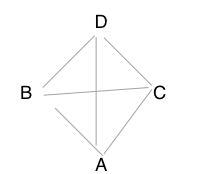
\includegraphics[clip,width=1\hsize]{img/PC_haichi.png}
          \caption{PC配置}
          \label{fig:relpos}
        \end{center}
      \end{minipage}
      \begin{minipage}{0.68\hsize}
        \begin{center}
          \caption{50回試行時の端末間距離計測結果}
          \begin{tabular}{l|rrrrr}
            \hline
            {\footnotesize  端末間}&{\footnotesize 平均}&{\footnotesize 標準偏差}&{\footnotesize 実測距離(m) }\\
            \hline
            {\footnotesize A-D }&{\footnotesize 11.71889953}&{\footnotesize 1.24793883}&{\footnotesize 11.10 }\\
            {\footnotesize B-D }&{\footnotesize 7.767573696}&{\footnotesize 0.583510141}&{\footnotesize 7.77 }\\
            {\footnotesize C-D }&{\footnotesize 6.72675737}&{\footnotesize 0.774180135}&{\footnotesize 6.72 }\\
            {\footnotesize A-B }&{\footnotesize 6.564537924}&{\footnotesize 1.067679838}&{\footnotesize 6.83 }\\
            {\footnotesize A-C }&{\footnotesize 7.300425749}&{\footnotesize 1.283308926}&{\footnotesize 6.93 }\\
            {\footnotesize B-C }&{\footnotesize 4.771470221}&{\footnotesize 0.664454607}&{\footnotesize 4.92 }\\
            \hline
          \end{tabular}
          \label{tab:estdistance}
        \end{center}
      \end{minipage}
    \end{tabular}
  \end{center}
\end{figure}



\section{DBAP法の有効性}

被験者の聴衆実験を行った.
被験者の向きの要因-45,0,45,90度,
距離要因として端末群の端から-1.15,0,1,2.31,4.62m,
音源位置を4箇所に用意し,音源位置を答えさせた.
実験結果を図\ref{fig:gosa},\ref{fig:hikenshaichi},\ref{fig:ongenichi}に示す.
距離が遠いと誤差があるものの,誤差は1メートル前後である.
端末数が少ない(4台)でDBAPをしてアレイの外にいる受聴者が音像を4台の中に感じたのは当然の結果である.
内部に入るとまったく定位できなくなった.
教室内で利用するときに,100人規模,20-30m平米の教室であれば,この程度の誤差は許容できる.


DBAP法の原理上,音のみかけの幅(ASW)と,音に包まれた感じ(LEW)が生じる\cite{ku-kanonkyo, onbasaigen, onkyoukougaku, 森本政之, 森本政之09, 森本政之90, 森本政之93, 崔瑛芝, 上杉信敏, 田中雅史}
もっと高密度に端末が分布している時のDBAPの効果が知りたい


\begin{figure}[p]
  \centering
  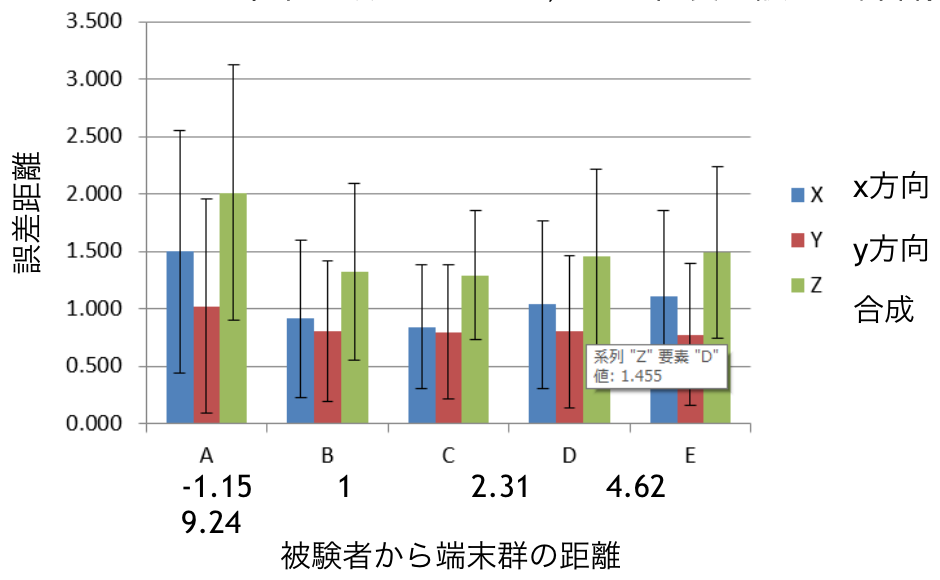
\includegraphics[clip,width=1.05\hsize]{img/bougurahu.png}
  \caption{誤差距離}\label{fig:gosa}
\end{figure}


\begin{figure}[p]
  \centering
  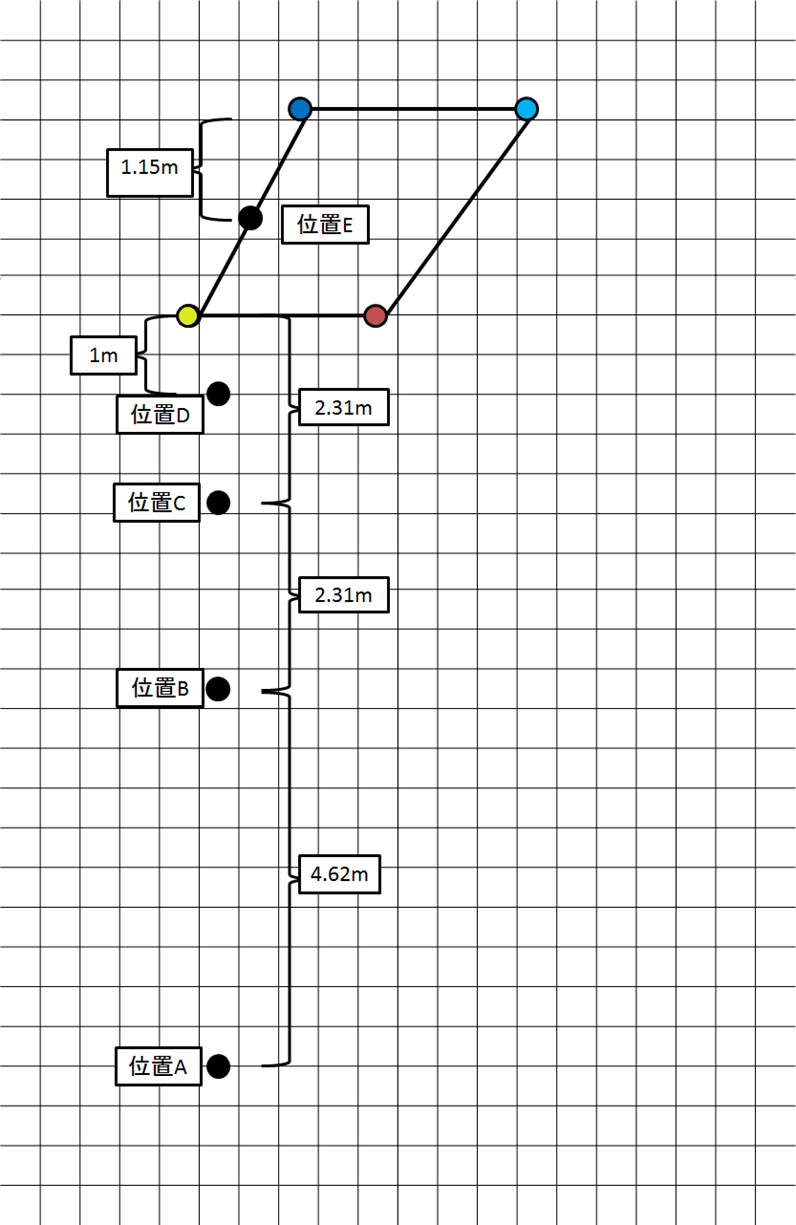
\includegraphics[clip,width=1.05\hsize]{img/hikenshaichi.png}
  \caption{被験者位置}\label{fig:hikenshaichi}
\end{figure}


\begin{figure}[p]
  \centering
  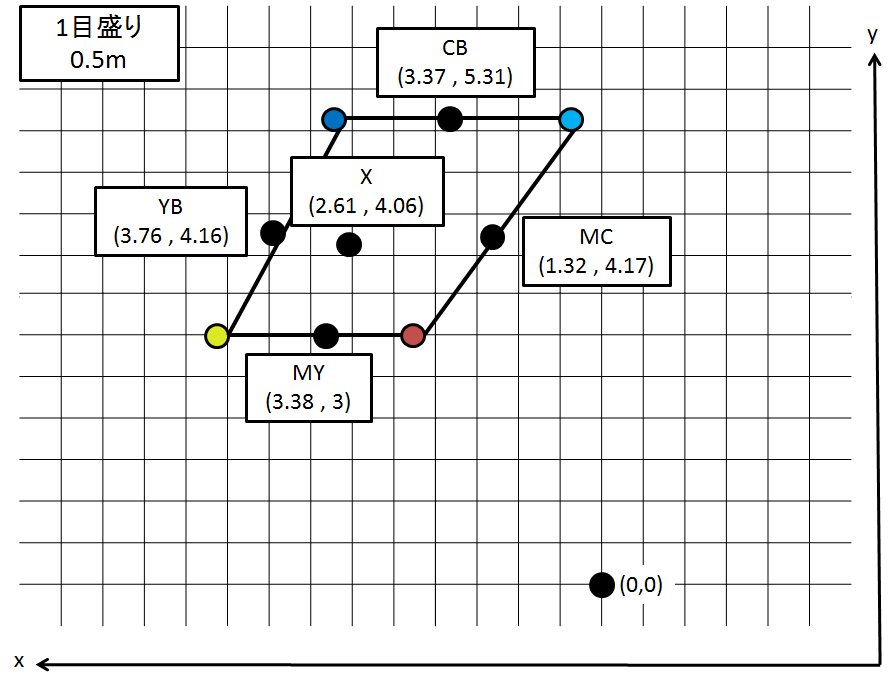
\includegraphics[clip,width=1.05\hsize]{img/ongenichi.png}
  \caption{音源位置}\label{fig:ongenichi}
\end{figure}




%\section{音圧校正手法の有効性}
%\section{クロックずれ校正手法の有効性}
%\section{隣接ノードでない端末間の各種手法の有効性}


\section{barker coded chirpについて}
以前使用していたbarker coded chirpによるパルスを利用した端末間距離測定の評価も行った.
MacBookAir13インチ3台を,1辺2mの正三角形に配置し,
先述のアルゴリズムにより各端末間距離を10回計測した.
表\ref{tab:estdistance}に,計測された各端末間の信号伝達時間と,その伝達時間から音速を340m/sと仮定したときの計測距離をそれぞれ示す.
最頻値はカーネル密度推定により求めた.

\begin{table}[p]\centering
  \caption{端末間距離計測結果}
  \label{tab:estdistance}
  \begin{tabular}{l|rrrrr}
    \hline
    端末間&平均(s)&最頻値(s)&中央値(s)&標準偏差&計測距離(m)\\
    \hline
    A-B&0.0061&0.0061&0.0061&0.00001&2.08\\
    A-C&0.0066&0.0067&0.0067&0.00013&2.27\\
    B-C&0.0057&0.0057&0.0057&0.00001&1.94\\
    \hline
  \end{tabular}
\end{table}


その結果,最大27cm(A-C間),最小6cm(B-C)の誤差にとどまった.
MacBookAir13インチの幅は30cm程度あるため,推定距離の誤差を考慮しても高精度に測距・同期できたと言える.
また,標準偏差も極めて低く,高確度に測定できていることが分かる.
この同期・測距の後,被験者1名に対して音源を各端末とも同一のボリュームで再生したところ,同一の音源として聴こえ,端末の三角形の内部に音像が定位された.
また,三角形の一辺が大きいと,受聴者がその三角形の外側の時には,みかけ音源の幅(ASW: auditory source width)が大きくなり,受聴者が三角形の内側の時に音に包まれた感じ(LEV: listener envelopment)を体験した.

  \chapter{考察}
%研究全体の考察
\begin{comment}
既知の問題としては,Nexus7が録音中に頻繁にバッファを取りこぼすことが挙げられる.

%![](img/nexus7_is_bad.png)

この現象によりパルスが到来した時刻が分からないので,上記手法が使えなかった.
原因はハードウェアにあるのかOSにあるのかブラウザの実装にあるのか不明であり,現在調査中である.
MacBookAirとMacBookPro間では同期に成功している.



他には,TDMAのみではN回の排他的パルス送信が必要で同期に時間がかかるという問題がある.
これにはスペクトル拡散を使っているのでCDMA(Code Division Multiple Access)化できる余地があるが,
今までの実験で,Nexus7ではGold符号でBPSKした信号が重なったときに,
分離検出できないという問題があったため,開発は滞っている.

\end{comment}

まず,本研究で狙いとするスマートデバイスを用いた音像定位手法として,
端末間同期において提案手法による高精度な同期・測距が実現した.
また,その同期を果たした複数端末による音像定位は,同一の音源として聞かせることができた.

受聴者からみた三角形のみかけの幅が大きい場合にASWが増加したのは,
ASWの要因である二つのノード間で両耳間相関度(ICC: interaural cross-correlation)が
%不可干渉
%インコヒーレントだからだと考えられる<<要出典>>.
小さかった\cite{morimoto95},もしくは,
もう一つの要因として初期側方エネルギー率が大きい,
つまり直接音の入射角度に対して垂直な成分の音圧レベルと直接音の音圧レベルの比が大きかった\cite{barron81}
と考えられる.
%という要因<<要出典>>も考えられる.
また,
三角形の内側の受聴者がLEVを体験したのは,
LEVの要因である前後エネルギー比\cite{suehiro06}
が小さくなったからと考えられる.


\section{barker coded chirpについて}
提案手法で使われるパルス圧縮がbarker coded chirpからM系列符号による直接拡散方式に変わった理由を述べる.

本来barker codeはそのままサイン波に適用し直接拡散して使うものであるが,
系列長が最大で13までしかないため,パルス圧縮に上限があった.
一方でchirp信号は引き伸ばせば引き伸ばすほどパルス圧縮されるが,サイドローブが大きくなるという問題を抱えていた.
そのため,この二つの手法を組み合わせて,短いup-chirpの繰り返しをbarker codeで拡散することで,
サイドローブを抑えながら圧縮する手法を試みた.
しかしながらこの手法は高周波成分において非線型歪みの影響を受けやすく,複数のピークが現れてしまうという問題を抱えていた.
%要図

一方で,M系列符号には系列長に制限がないため,そのような手法を必要とせず,直接拡散方式が利用できる.
以前の実装は私がbarker codeによるパルス圧縮を知った時点で,まだM系列符号を知らなかった故のものであり,
M系列符号が使える現在,そのようなハイブリット手法を使う理由はない.

  \chapter{結論}
\section{本研究の成果}
%と,限定された点を明らかにしたり,
%さらに改善されるべき点を述べる

以上の通り,スマートデバイスを用いて
DBAP法を用いたスピーカアレイを構築できることを示した.


\section{本研究の展望}
%どうしたらもっとよくなるか
%どうしたら残ってる問題を解決できそうか.

\subsection{相対位置推定結果が回転・反転する問題}



ダイレクトパスがない時に同期性能落ちる.
端末間に障害物があると音波が回折して伝搬する.
コンクリート壁などの反射波の方がエネルギー大きくなる、あるいは非線形歪みの影響がある\cite{nonlinear}.
微弱な先行波を捉える手法の必要性があるが,非線形歪みと反射音,回折音をどう区別するかの問題が残っている.
ハードウェアや環境に応じて2端末間のインパルス応答は毎回異なるため識別は困難である.


\subsection{相対位置推定結果が回転・反転する問題}

相対位置推定の結果が理解できない.
問題設定上,回転や鏡面反転した解が出てきてしまう.
これは,相対位置を推定している以上防ぐことができない.
そのため,ユーザが手で修正するためのUIを実装する必要がある.
他にも,2台の端末の位置を固定してしまい推定から外してしまえば,回転・反転は防ぐことができる.


\subsection{相対位置推定アルゴリズムの解が収束していない}

相対位置推定の結果が現実の位置を反映できていない.
これは,最急降下法の解が収束していないのが原因である.
推定アルゴリズムを改良する必要がある.


\subsection{音圧校正}

端末ごとに音圧出力が異なる問題もある.
これは,スピーカアンプの出力の差が原因である.
これには,互いに観測したパルスの振幅から距離減衰を推定し,相対的な音圧比率を計算することができる.
(図:\ref{fig:spc})

\begin{figure}[p]
  \centering
  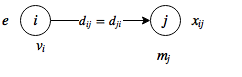
\includegraphics[clip,width=1.05\hsize]{img/sound_pressure_calibration.png}
  \caption{2端末間の振幅減衰のモデル}\label{fig:spc}
\end{figure}

$$
ev_i \frac{1}{d_{ij}}m_j = x_{ij}
$$

$$
\frac{v_j}{v_k} = \frac{x_{ij}d_{ij}}{x_{kj}d_{kj}}
$$

これもこのモデルが成り立つか実験が必要である.


\subsection{システムクロックの校正}

システムクロックの差に依存するズレがある.
これを解決するには2端末間でシステムクロックの差を検出すればよい.
具体的には2回パルス受信してサンプリング数の差を計測すれば良い(図\ref{fig:ps2}).

$$
\frac{S_B}{S_A} = \frac{i+d}{i}
$$

\begin{figure}[p]
  \centering
  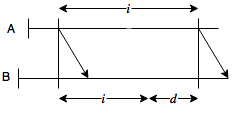
\includegraphics[clip,width=1.05\hsize]{img/phase_shift2.png}
  \caption{再同期}\label{fig:ps2}
\end{figure}

\subsection{パルス検出できない端末間で同期}
多段同期すればよい
クロック校正も多段校正できる
音圧校正も多段校正できる(図\ref{fig:nt})

\begin{figure}[p]
  \centering
  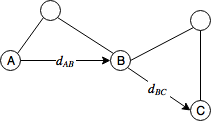
\includegraphics[clip,width=1.05\hsize]{img/network_topology.png}
  \caption{再同期1}\label{fig:nt}
\end{figure}



端末 $A$ を基準に音圧校正を考えると

$$
\frac{v_B}{v_A} = \frac{x_{iB} d_{iB}}{x_{AB}d_{AB}} \\
\frac{v_C}{v_B} = \frac{x_{iC} d_{iC}}{x_{BC}d_{BC}} \\
$$

であるので

$$
\frac{v_C}{v_A} =
\frac{v_B v_C}{v_A v_B} =
\frac{x_{iB} x_{iC} d_{iB} d_{iC}}{x_{AB} x_{BC} d_{AB} d_{BC}}
$$

とすれば端末 A と端末 C の出力比率を求められる.
要実験である.

また,同期に関しては,
時刻の基準となる
端末 $A$ がパルスを発した時間を $t_{AA}$ として
そのパルスが端末 $B$ に届いた時間は $t_{AB}$ とする.
また,
端末 $B$ がパルスを発した時間を $t_{AB}$ として
そのパルスが端末 $C$ に届いた時間は $t_{BC}$ とする.
そしてそれぞれの伝達時間を $d$ とすると図\ref{fig:rd}のようになる.

\begin{figure}[p]
  \centering
  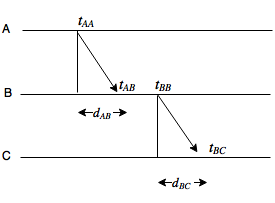
\includegraphics[clip,width=1.05\hsize]{img/rel_delay.png}
  \caption{再同期2}\label{fig:rd}
\end{figure}

このとき,まず端末 $C$ は端末 $B$ と同期して,
その後端末 $B$ と端末 $A$ の時刻ずれ情報をもとにさらに端末 $A$ との同期ができる.



\subsection{パルス回数の問題}
現在の提案手法では同期に時間がかかるのでリアルタイム同期できるようにしたい.
N台の同期にN回パルス必要という問題もある.
これには,TDMAだけでなくCDMA(符号分割多元接続)も試した.
シミュレーションではうまく機能したが,
実際に試すとパルスが重なったときに信号をうまく分離できない問題があった.
これも拡散符号の非線形歪みの影響と考えられる.
ところで,音圧校正・同期を考えなければ,つまり測距だけならば,パルスは3台が1回ずつ放てば十分である.
これはGPSと同じ仕組みであり,3台の端末の相対位置さえわかってしまえば,
他の端末はその3台からの相対距離がわかれば三角測量の要領で相対位置が算出できるからである.
この手法に合わせて同期手法を提案手法とは異なる結合振動子系のような適応的アルゴリズムにすることで,システムクロックのずれにも対応できるようになる.
しかしながら,音圧校正のためには現在の手法では全ての端末が音を出す必要がある問題が残されている.


\subsection{位置変更による再同期の必要性}

端末が動くと再同期が必要という問題もある.
この原因は同期と測距を同時にしているからである.
逆に言えば,測距と同期とは別の手法を用いればよい.
例えば,GPSと同じように,位置固定した連続パルス発信端末を導入すればよい.
これにより,リアルタイム測距は可能になる.
同期に関してはも結合振動子系のような適応的なアルゴリズムを採用すれば,システムクロックのずれにも対応できるようになる
しかしながら,音圧校正のためには現在の手法では全ての端末が音を出す必要がある問題が残されている.


\subsection{計算量・計算時間削減のための最適化}
相互相関の計算に離散フーリエ変換ではなく離散コサイン変換を使うことで計算量を削減できる可能性がある.
しかしながら,高速離散フーリエ変換を高速離散コサイン変換に置き換えたことによる計算量の削減は高々O(n)であり、負荷改善のために導入するには最適化の時期が早すぎると思われる.


\section{本研究の総括と結論}

教室空間における複数の個人所有のスマートデバイスを用いてスピーカアレイを構築し,DBAP法を用いた音像定位するシステムを提案した・
各端末を音声パルスを用いることで時刻同期し,位置を推定し,仮想音源を配置できることを示した.
これにより教室空間における新しい音声コミュニケーション手法を実現した.

  \begin{thebibliography}{99}
%\begin{bibliography}{}
\addcontentsline{toc}{chapter}{参考文献}

% intro
\bibitem{11ubi}       Yu Zheng, Yanchi Liu, Jing Yuan, and Xing Xie, Urban Computing with Taxicabs, In Proc. of Ubicomp 2011, pp. 89--98, 2011.
\bibitem{surechigai}  末廣 創,佐藤 文明,すれ違い通信による情報伝搬モデルの特性評価,情報処理学会全国大会講演論文集 第72回(ネットワーク), 155-156, 2010-03-08, 2010.
\bibitem{clicker}     April R. Trees, and Michele H. Jackson. The learning environment in clicker classrooms: student processes of learning and involvement in large university‐level courses using student response systems. Learning, Media and Technology, vol.32, no.1, pp.21--40, 2007.
\bibitem{imakiku}     株式会社天問堂, Imakiku, \url{http://tenmondo.com/products/imakiku/index.html} (2015時点)
\bibitem{twitter}     後藤 真孝, WISS 2010 と WISS 2011 での改革, コンピュータソフトウェア (日本ソフトウェア科学会誌), Vol.29, No.4, pp.3--8, 2012.

% related
\bibitem{kawagoe14} 河越嵩介,神場知成,田中二郎.位置情報を利用した携帯端末への音声情報配信,情報処理学会第76回全国大会,4ZA-2,2014.
\bibitem{wfs}       Berkhout, Augustinus J., Diemer de Vries, and Peter Vogel. "Acoustic control by wave field synthesis." The Journal of the Acoustical Society of America 93.5 (1993): 2764-2778.
\bibitem{hoa}       Daniel, Jérôme. "Spatial sound encoding including near field effect: Introducing distance coding filters and a viable, new ambisonic format." Audio Engineering Society Conference: 23rd International Conference: Signal Processing in Audio Recording and Reproduction. Audio Engineering Society, 2003.
\bibitem{sfc}       Ise, Shiro. "A principle of sound field control based on the Kirchhoff-Helmholtz integral equation and the theory of inverse systems." Acta Acustica united with Acustica 85.1 (1999): 78-87.
\bibitem{paramsp}   青木茂明,清水一博,伊藤昂輝.パラメトリックスピーカを用いた再生時の音像定位.信学技報 EA研究会,vol.114,no.423, pp.33--38, 2015.
\bibitem{shibata13} 柴田一暁, 小野順貴, 亀岡弘和. 音の発信を利用したスマートフォンアレイの機器位置推定. 音講論 (秋), pp.591--592, 2013.
\bibitem{shibata14} 柴田一暁, 小野順貴, 亀岡弘和. 音の発信を利用したキャリブレーションに基づくアドホックマイクロホンアレイによる音源定位. 音講論 (春), pp. 707--710,2014.
\bibitem{Aoshima}   N. Aoshima, Computer-generated pulse signal applied for sound measurement, J. Acoust. Soc. Am., vol.69, no.5,1484--1488, 1981.


% system
\bibitem{dbap}      Trond Lossius, Pascal Baltazar, and Theo de la Hogue. DBAP–distance-based amplitude panning. Proc of ICMC 2009, pp.489--492, 2009.
\bibitem{tpsn}      Ganeriwal, Saurabh, Ram Kumar, and Mani B. Srivastava. "Timing-sync protocol for sensor networks." Proceedings of the 1st international conference on Embedded networked sensor systems. ACM, 2003.
\bibitem{Haas}      (After Helmut Haas's doctorate dissertation presented to the University of Gottingen, Gottingen, Germany as "Über den Einfluss eines Einfachechos auf die Hörsamkeit von Sprache;" translated into English by Dr. Ing. K.P.R. Ehrenberg, Building Research Station, Watford, Herts., England Library Communication no. 363, December, 1949; reproduced in the United States as "The Influence of a Single Echo on the Audibility of Speech," J. Audio Eng. Soc., Vol. 20 (Mar. 1972), pp. 145-159.)
\bibitem{pof}       Horner, Joseph L., and Peter D. Gianino. "Phase-only matched filtering." Applied optics 23.6 (1984): 812-816.
\bibitem{overwrap}  Rabiner, Lawrence R., and Bernard Gold. "Theory and application of digital signal processing." Englewood Cliffs, NJ, Prentice-Hall, Inc., 1975. 777 p. 1 (1975).

\bibitem{umezu11}   梅津直貴, 井ノ上寛人, 堀内恒, 佐藤美恵, 小黒久史, 春日正男.空間把握性に注目した音響案内システムの開発に関する研究.映像情報メディア学会技術報告 vol.35, no.39, pp.41--44,2011.
\bibitem{onzou}     平原達也, 蘆原郁, 小澤賢司, 宮坂榮一, 音と人間, 日本音響学会編, コロナ社, 2013.


\bibitem{raylei1877}
Lord Rayleigh, Acoustical Observations I,
Philosophical Magazine Series 5, vol. 3, Issue 20, pp.456--464, 1877.
%http://www.tandfonline.com/doi/abs/10.1080/14786447708639268?journalCode=tphm16
\bibitem{raylei1907}
Lord Rayleigh, On our perception of sound direction,
Philosophical Magazine Series 6, vol. 13, Issue 74, pp.214--232, 1907.
%http://www.tandfonline.com/doi/abs/10.1080/14786440709463595#abstract
%[Lord Rayleigh: On our perception of sound direction, Phil.Mag, 13,6th series,pp.214-232(1907)]
\bibitem{komatsu2014}
小松潤也, 塩田茂雄, センサ協調位置推定: 相互多辺測量法と多次元尺度構成法の精度比較, 信学技報, ASN 114(65), pp.127--132, 2014.
\bibitem{senkouon}
H. Haas, The Influence of a Single Echo on the Audibility of Speech,
Journal of Auditory Engineering Society, vol. 20, Issue 2, pp.146--159, 1972.
%http://www.aes.org/e-lib/browse.cfm?elib=2093
%播摩敏雄, 安倍幸治, 高根昭一, 曽根敏夫, 音像定位における先行音効果とエコー知覚の限界に関する考察, HIP 104(526), pp.13--18, 2004.
%http://ci.nii.ac.jp/els/110003272588.pdf?id=ART0003775596&type=pdf&lang=jp&host=cinii&order_no=&ppv_type=0&lang_sw=&no=1451791039&cp=
\bibitem{vbap}
Vikke Pulkki, Virtual Sound Source Positioning Using Vector Base Amplitude Panning, Journal of Audio Engineering Society, Vol. 45, Issue 6, pp.456--466, 1997.

%Trond Lossius, et al., DBAP - Distance based amplitude panning, International ComputerMusic Conference (ICMC). Montreal, 2009.
\bibitem{self_ac}
伊納洋祐, 吉田侑矢, 米澤朋子,	複数端末の音響的位置推定と同期による空間音響環境構築システムの提案,	ASJ 2014 autumn,	pp.1439--1440,	2014.
\bibitem{seigoufilter}
滑川俊彦,奥井重彦,衣斐信介,通信方式(第二版),森北出版,2012.
\bibitem{pulsecompress}
近藤倫正,, 実森彰郎,大橋由昌,計測・センサにおけるディジタル信号処理,昭晃堂,1993.
\bibitem{chordalg}I. Stoica, R. Morris, D. Karger, M. F. Kaashoek, H. Balakrishnan.Chord: A scalable peer-to-peer lookup service for internet applications.ACM SIGCOMM Computer Communication Revies, vol. 31, issue 4, pp.149--160,2001.
\bibitem{morimoto95}
Morimoto, Masayuki, and Kazuhiro Iida. A practical evaluation method of auditory source width in concert halls. Journal of the Acoustical Society of Japan (E) vol.16, no.2, pp.59--69, 1995.
\bibitem{barron81}
M. Barron, and A. H. Marshall. Spatial impression due to early lateral reflections in concert halls: the derivation of a physical measure. Journal of Sound and Vibration, vol.77, no.2, pp.211--232, 1981.
%音響工学基礎論
\bibitem{suehiro06}
末廣大地, 翁長博, 池田哲朗. 音楽ホールにおける音に包まれた感じに対応する物理指標の検討. 日本建築学会環境系論文集,no.599, pp.1--7, 2006.
\bibitem{cheun97}
Kyungwhoon Cheun. Performance of Direct-Sequence Spread-Spectrum RAKE Receivers with Random Spreading Sequences.
IEEE Transactions on communications, vol.45, no.9, pp.1130--1143, 1997.
\bibitem{honer84}
J. L. Horner, P. D. Gianino. Phase-only matched filtering. Applied optics, vol.23, no.6, pp.812--816, 1984.
%C言語によるディジタル無線通信技術
%アコースティック・イメージング
%原理が分かる・現場で使える信号処理

%http://sonove.angry.jp/about_localization.html
%http://acousticslab.org/psychoacoustics/PMFiles/Module07b.htm

\end{thebibliography}
%\end{bibliography}{}

  \chapter*{謝辞}
\addcontentsline{toc}{chapter}{謝辞}

謝辞はだいたい1ページぐらい.お世話になった人すべて取り上げたほうがいい,
ただし,同僚は除いてもよいかな.

  \appendix

\def\thesection{付録\Alph{section}\\}


\chapter{納豆の菌糸の動画キャプチャ}


\begin{figure}[tb]\centering
\epsfxsize=10cm\epsffile{eps/natto.eps}
\caption{菌糸,33日目}\label{fig:kinshi33}
\end{figure}

\chapter{納豆を嫌がる人口比率と都道府県}

\begin{table}[tb]\centering
%\epxfxsie=10cm\epsffile{}
\caption{都道府県と納豆}\label{tab:todoufuken}
\begin{tabular}{lcc}
\hline
都道府県&すき&きらい \\ 
\hline
神奈川県&80&20 \\ 
大阪府&20&80 \\ 
\hline
\end{tabular}
\end{table}

  \chapter*{発表文献リスト}
\addcontentsline{toc}{chapter}{発表文献リスト}

\begin{itemize}

  \item[] ジャーナル論文
  \begin{enumerate}
    \item 伊納洋佑, et al. 複数の携帯端末による教室空間の空間音響環境構築手法の検討. 研究報告コンピュータビジョンとイメージメディア (CVIM), 2014, 2014.7: 1-4.
    \item 伊納洋佑, et al. 複数の携帯端末による教室空間の空間音響環境構築手法の検討 (人体・動作の認識と理解, 福祉と共生, 国際会議報告). 電子情報通信学会技術研究報告. MVE, マルチメディア・仮想環境基礎, 2014, 113.403: 41-44.
    \item 岡本直也; 伊納洋祐; 米澤朋子. ディジタル画像への温感付与による非実体の体感システム提案 (第 109 回ヒューマンインタフェース学会研究会 高齢者, 障がい者支援技術および一般). ヒューマンインタフェース学会研究報告集, 2014, 16: 33-36.
    \item 河口拓貴, et al. 上体の重心移動を伴う身体動作による音楽演奏時のリズム生成手法の提案 (人体・動作の認識と理解, 福祉と共生, 国際会議報告). 電子情報通信学会技術研究報告. PRMU, パターン認識・メディア理解, 2014, 113.402: 49-52.
    \item 石野力, et al. 複数パラメトリックスピーカを用いた一対多コミュニケーション手法の提案 (人体・動作の認識と理解, 福祉と共生, 国際会議報告). 電子情報通信学会技術研究報告. MVE, マルチメディア・仮想環境基礎, 2014, 113.403: 53-58.
    \item 石野力; 伊納洋祐; 米澤朋子. 空間指向性を含む繰り返し音楽の制御と演奏効果の検証. 情報処理学会研究報告.[音楽情報科学], 2015, 2015.18: 1-6.
    \item 中祐介, et al. 身体動作・環境音のオノマトペを含むテキストコミュニケーション手法の検討 (特集論文 「いい加減」なインタフェース) ヒューマンインタフェース学会論文誌 The transactions of Human Interface Society 17(1-4), 97-106, 2015
  \end{enumerate}

  \item[] 国際会議論文
  \begin{enumerate}
    \item hoge
  \end{enumerate}

  \item[] 国内会議論文
  \begin{enumerate}
    \item huga
  \end{enumerate}

  \item[] その他
  \begin{enumerate}
    \item hige
  \end{enumerate}

\end{itemize}




\end{document}
